\clearpage
\section{Ekonomický koloběh a funkce trhů. Úloha ceny v tržní ekonomice.}

\subsection{Ekonomický koloběh}
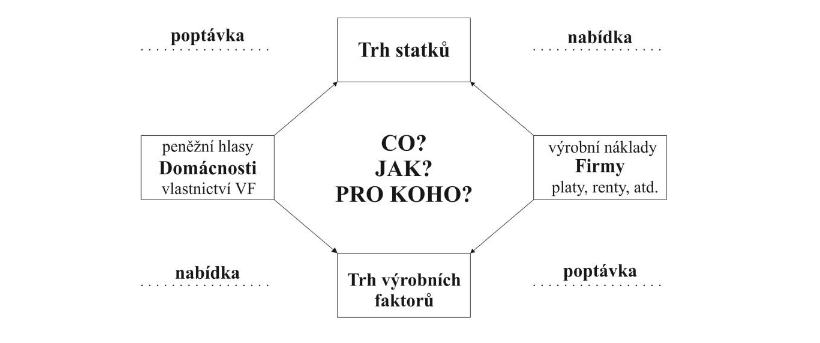
\includegraphics[width=16cm]{images/kolobeh.png}

\subsection{Funkce trhů}
\begin{itemize}
    \item Hledání odpovědí na otázky:
    \begin{itemize}
        \item \textbf{Co} vyrábět, rozhodováno peněžními hlasy (co se bude dobře prodávat)
        \item \textbf{Jak} vyrábět, soutěž mezi výrobci rozhoduje o nejlepším postupu
        \item \textbf{Pro koho} vyrábět, jak bude produkt rozdělen mezi jednotlivce nebo skupiny lidí
    \end{itemize}
    \item Dokáže na to odpovědět dokonale konkurenční trh, což je jen model
\end{itemize}

\subsection{Úloha ceny v tržní ekonomice}
\begin{itemize}
    \item Informační funkce - když se stane výrobní zdroj vzácnější, zvýší se cena
    \item Motivační funkce - Snaha ušetřit, spotřeba méně vzácných výrobků
    \item Alokační funkce - cenové informace -> přemístění výrobních zdrojů
\end{itemize}